%%%%%%%%%%%%%%%%%%%%%%%%%%%%%%%%%%%%%%%%%%%%%%%%%%%%%%%%%
%%%%%%%%%%%%%%%%%%%%% author:BrowningWan %%%%%%%%%%%%%%%%
%%%%%%%%%%%%%%%%%%%%% part:4.0-4.3       %%%%%%%%%%%%%%%%
%%%%%%%%%%%%%%%%%%%%%%%%%%%%%%%%%%%%%%%%%%%%%%%%%%%%%%%%%

\chapter{数值优化}
\label{chap:4}

    机器学习算法通常都需要大量的数值计算。数值计算通常指的是解决数学问题的算法(例如通过迭代的过程来更新对解的估计),而不仅仅指为了解出正确解得到的公式。常见的操作包括优化计算(找到对应最小化或最大化函数值的参数)和线性方程组的求解。对数字计算机来说,即使计算只涉及实数的函数也是困难的,因为实数无法在有限内存下精确表示(因为要离散化)。

\section{上溢和下溢}
    在数字计算机上实现连续数学计算的基本困难是,我们需要通过有限位数的数字量(离散值)来表示无限多的实数(连续值)。这意味着我们在计算机中表示实数时,几乎都会引入一些近似误差。在绝大多数情况下,这仅仅是舍入误差。如果我们不考虑最小化舍入误差的逐渐累积(链式法则),那么我们设计的理论上可行的算法可能不会在实践中有比较好的效果。

一种特别的毁灭性舍入误差是下溢。通常当接近零的数(非常小的数)被四舍五入为零时发生。许多函数会在其参数为零而不是一个很小的正数时才会表现出质的不同。例如,我们通常要避免除以零(一些软件环境将在这种情况报错,有些会返回一个非数字(not-a-number)的占位符)或取零的对数(这通常被视为-$\infty$,进一步的算术运算会使其变成非数字)。

另一个极具破坏力的数值错误形式是上溢。当特别大的数被近似为+$\infty$或-$\infty$时发生(通常因为变量位数不够溢出)。进一步的运算通常将这些无限值变为非数字量。必须对上溢和下溢问题进行数值稳定的一个例子是softmax函数。Softmax函数经常用于预测与多点分布相关的概率,其函数定义为:

\begin{equation}
	\mathop{\mathrm{softmax}}(x)_i=\frac{exp(x_i)}{\sum_{j=1}^nexp(x_j)}
\end{equation}

考虑一下当所有$x_i$都等于某个常数时会发生什么。从理论分析上说,我们可以发现所有的输出都应该为$\frac{1}{n}$。从数值计算上说,当该常数很大时,这可能不会发生。如果该常数是很小的负数,$exp(x_i)$就会发生我们刚才讲的下溢。这意味着softmax函数的分母会变成0,所以最后的结果是一个未定义的量。当该常数是非常大的正数时,$exp(x_i)$将会发生上溢,再次导致整个表达式未定义。上述两个问题都能通过引入一个新变量$z=x+maxx_i$,计算新的softmax(z)解决。通过简单的代数计算就能够证明我们上述的操作并不会使输出的函数值发生改变。由于减去了$maxx_i$项,使得至少有一项输入计算后为0,这就排除了发生上溢的可能性。同样地,分母中至少有一个值为1的项,也排除了因分母被零除而导致下溢的可能性。

仍有一个小问题存在。如果分子发生下溢,将会导致整个计算式被计算为0。举个例子,如果我们要计算$logsoftmax(x)_i$,我们先计算$logsoftmax(x)_i$,然后此时呢它发生了下溢,然后将结果0回传到了对数函数,我们就得到了最终结果-$\infty$(很明显是个错误的结果)。

在大多数情况下,我们没有明确地对实现本书描述的各种算法时所涉及的数值考虑进行详细说明。使用比较底层的库开发的读者在实现自己算法时应当牢记数值问题。本书的大多数读者可以简单地依赖一些保证稳定的底层库。在某些情况下,这些库可以在我们•实现一个新的算法时自动保持数值稳定。Theano就是这样一个底层库,它能自动检测并稳定深度学习中许多常见的数值不稳定的表达式。


\section{差条件数}

条件数表明函数相对于输入的微小变化而变化的激烈程度。对于轻微扰动的输入而迅速改变的函数对于科学计算来说是可能是有问题的,因为输入中的舍入误差可能导致输出的巨大影响(蝴蝶效应)。

考虑一个函数$f(x)=A^{-1}x$当A为方阵时,该方阵可以特征值分解。该函数条件数为:

\begin{equation}
\max_{i,j}|\frac{\lambda_i}{\lambda_j}|
\end{equation}

这是最大特征值和最小特征值之比的模。当该条件数很大时,矩阵求逆对输入的误差特别敏感。

这种敏感性是矩阵本身的固有属性,而不是矩阵求逆期间舍入误差的结果。即使我们乘以完全正确的矩阵逆,有差条件数的矩阵也会放大预先存在的误差。在实践中,该错误将与求逆过程本身的数值误差进一步复合,影响我们结果的正确性。

\section{基于梯度的优化算法}

大多数深度学习算法都或多或少地涉及到了不同形式的优化方法。优化方法指的是通过改变自变量输入的数值以最小化或最大化的对应函数输出的过程。我们通常以最小化函数输出指代大多数最优化问题。函数最大化输出可经由求对应反函数的最小化输出来实现。

我们把希望取得最小化或最大化的函数叫做目标函数。当我们对其进行最小化时,我们也把它叫做代价函数,损失函数或误差函数。虽然有些机器学习著作赋予这些名称特殊的意义,但在这本书中我们会交替使用这些术语。

我们通常使用一个上标符号*来表示对应最小化或最大化函数的自变量输入值。例如:

\begin{equation}
x^*=argminf(x)
\end{equation}

我们假设读者已经熟悉微积分,但是这里我们仍然简要地回顾下微积分如何与优化联系起来。

图\ref{fig:4_1}
\begin{figure}[htbp] %  figure placement: here, top, bottom, or page
   \centering
   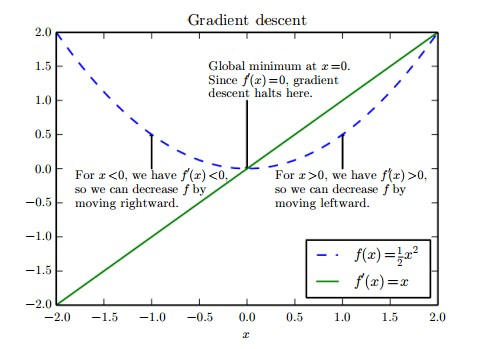
\includegraphics[width=6in]{fig/chap4/4_1.jpg} 
   \caption{Title:梯度下降
左:对于输入x小于0的部分,此时导数小于0,所以我们能通过向右移动来提升函数值;
中:对于输入x等于点部分,此时导数等于0,该处取得极小值,梯度下降在该点停止;
右:对于输入x大于0的部分,此时导数大于0,所以我们能通过向左移动来提升函数值;}
   \label{fig:4_1}
\end{figure}

图4.1:一个函数的导数可以用来跟踪函数使其下降到最小值的例子。 该方法被称为梯度下降。

假定我们有一个函数y=f(x), 其中和是实数。该函数的导数记为f'(x)或$\frac{\partial y}{\partial x}$.

导数f'(x)代表该函数f(x)在点x处的斜率。换句话说,它表明需要如何使输入产生小变化以在输出获得相应的变化:

\begin{equation}
f(x+\varepsilon)\approx f(x)+\varepsilon f'(x)
\end{equation}

因此导数对于最小化一个函数很有用,因为它告诉我们如何改变输入来调整我们的输出。例如,我们知道对于足够小的$\varepsilon$来说,$ f(x-\varepsilon sign(f'(x)))$是比小的。因此我们可以将往梯度的反方向移动一小步来减小输出值。这个方法被叫做梯度下降法。图4.1向我们举了个例子。

当f'(x)=0时导数不能提供移动的方向信息。在f'(x)=0处的点被称为$\emph{临界点}$或者$\emph{平稳点}$。$\emph{局部极小值}$就是指f(x)要小于附近点,所以不可能在该点通过向旁边(左右)移动来进一步使函数值下降。$\emph{局部极大值}$就是指f(x)值要大于附近点,所以不可能在该点通过向旁边(左右)移动来进一步使函数值上升。

一些临界点既不是极大值也不是极小值,称之为$\emph{鞍点}$,见图4.2的举例是各种形式的临界点。

图\ref{fig:4_2}。
\begin{figure}[htbp] %  figure placement: here, top, bottom, or page
   \centering
   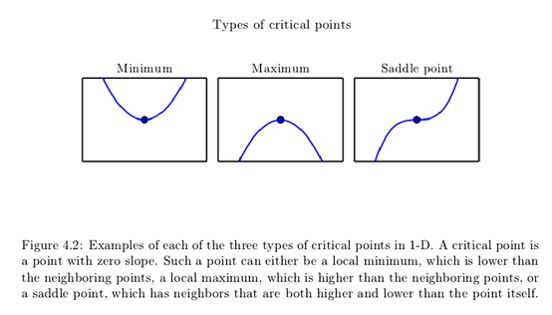
\includegraphics[width=6in]{fig/chap4/4_2.jpg} 
   \caption{左 极小值 中 极大值 右 鞍点
图4.2 在一维空间中三种临界点的例子,临界点指的是斜率为零的点。比附近点都小的点可以作为局部极小值,比附近点都大的点可以作为局部极大值,或者同时不算极大值极小值的鞍点。}
   \label{fig:4_2}
\end{figure}

当一个点是整个f(x)最低值时它就是$\emph{全局极小值}$,对于一个函数可能有唯一一个(全局极小值,即最小值)或者多个局部极小值。局部最小值也可能不是全局极小,在深度学习的背景下,我们优化并不处于最优点的具有多个局部极小值的函数和被许多鞍值包围的非常“平坦”的函数。这些都使得我们的优化变得十分困难,尤其当函数的输入是多维的时候。所以我们经常勉强接受一个很低的f值(一个局部极小值),但并不是在任何意义上的最小值。见图4.3中举例。

我们经常按如下方法处理多端输入的最小函数:f:$R^n$=R。为了使“最小化”有意义,必须只有一个(标量)输出。

对于多输入的方程,我们必须引入$\emph{偏导数}$概念。偏导数${}^{\varepsilon}_{\varepsilon x_i}\textrm{f(x)}$描述了函数f在点x处只在变量$x_i$增加时的变化。梯度的概念可以推广到导数,就是说导数可以看做一个向量:的梯度就是一个包括所有偏导数的向量,表示为$\nabla_x f(x)$。梯度的单元i是关于$x_i$的偏导数。在多个维度中临界值就是每个梯度元素都为零的点。

在u方向的方向导数就是(一个单位向量)就是f在u方向的导数。换句话说,方向导数就是关于α的方程f(x+αu),当α=0的导数。根据链式法则,我们可以认识到${}^{\partial}_{\partial\alpha}\textrm{f(x+$\alpha$u)}=u^T \nabla_x f(x)$

为了最小化f,我们愿意找到f降低最快的方向。我们可以用方向导数实现:
 
当$\theta$是u和梯度之间的夹角时。将其带入$\left \| u \right \|_2$=1中,并忽略与u变化无关的因素。带入不依赖,于是原式简化为$min_u \cos\theta$。当u与梯度反向时,该式取得最小解。换句话讲,梯度指向直接的上升,负梯度指向直接下降。我们可以通过反梯度方向移动降低值。这被称为最快下降法和梯度下降法。

图\ref{fig:4_3}。
\begin{figure}[htbp] %  figure placement: here, top, bottom, or page
   \centering
   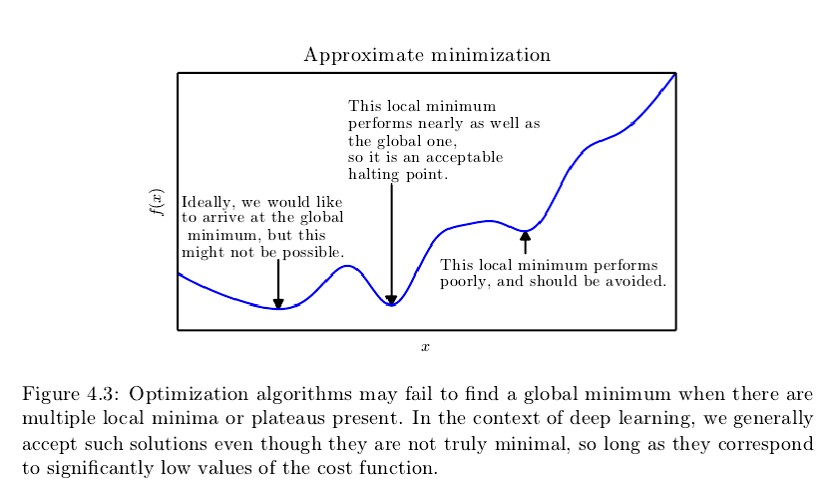
\includegraphics[width=6in]{fig/chap4/4_3.jpg} 
   \caption{图4.3:多个局部最小值或者平台出现时最优化算法有可能不能够找到局部最小值。在深度学习领域,我们一般接收即便不是真是最小值的解,只要它在价值函数中有对应的显著的最小值}
   \label{fig:4_3}
\end{figure}

最快下降法引入了一个新的变量:

\begin{equation}
x'=x-\epsilon\nabla_x f(x)
\end{equation}

在这里$\epsilon$是学习速率,一个正的标量决定了步长。我们可以从几个不同的方法选择$\epsilon$。一个流行的方法就是将$\epsilon$设定为一个小量。有时我们可以通过使方向导数消失来解决步长大小。另一种方式是去给定几个$\epsilon$的值,并评价$f(x-\epsilon\nabla_x f(x))$,然后去选一个使得目标函数值最小的值。最后一种策略叫做线性搜索。

当每一个单元的梯度都为零时最快下降法收敛(或者在练习时,非常接近0)。在一些情况下,我们能够避免运行这种迭代算法,并且通过解决关于x方程$\nabla_x f(x)=0$直接跳到临界点。

尽管梯度下降在连续区间内的优化是有限制的,一般概念上向更好结构的小移动(就是很小的移动)是可以推广到离散域内的。上升的离散参量目标函数被称作$\emph{目标法}$。

\section*{“超越”梯度的计算:(雅克比矩阵和海森矩阵)}

有时我们需要找到所有输入和输出都是响亮的函数的偏导数。包含那些全部偏导的行列式称为雅克比矩阵。特定的,如果我们有函数f:$R^m\to R$,那么的雅克比矩阵为$J\epsilon R^{n*m}$被定义为$J_{i,j}=\frac{\partial}{\partial x_j}f(x_i)$

我们有时也对导数的导数感兴趣,这被称作$\emph{二阶导数}$。比如,函数f:$R^n\to R$,对$x_j$的导数再对$x_j$求导被表示为$\frac{\partial^2}{\partial x_i\partial x_j}$f.在单一的方向,我们可以将$\frac{d^2}{dx^2}$f表示为f"(x).二阶导告诉我们当改变输入量时一阶导的变化。这是十分重要的,他告诉我们仅靠梯度变化是否能够达到我们想要的增益。我们可以认为二阶导数是测量$\emph{曲率}$。假设我们有一个二次函数(许多在练习中出现的函数不是二次函数,但是至少在局部可以良好近似为二次的)。如果这个方程有一处二阶导数为零,那这里没有曲率。这是一条完美的斜直线,他的值能够仅凭梯度进行估计。如果梯度是1.那么我能可以通过负梯度设定步长$\epsilon$,并且价值函数会随着$\epsilon$而降低。如果二次导数是负的,那么函数曲线向下弯曲,所以价值函数的实际下降会多于$\epsilon$。最终,如果二次导数是正的,函数曲线向上弯曲,价值函数的降低会小于$\epsilon$。见图4.4能够看出曲率影响价值函数的预测值与真实值的不同线形和关系。

当我们的函数有多个输入维度时,就有许多二阶导数。这些导数可以被收在一个称作黑森的矩阵中。海森矩阵H(f)(x)被定义为

\begin{equation}
H(f)(x)_{i,J}=\frac{\partial^2}{\partial x_i\partial x_j}f(x)
\end{equation}

相当于是海森是雅克比的梯度。
在任何地方的二次偏导数都是连续的,微分项可以调换,举例说它们的顺序可以写成:

图\ref{fig:4_4}。
\begin{figure}[htbp] %  figure placement: here, top, bottom, or page
   \centering
   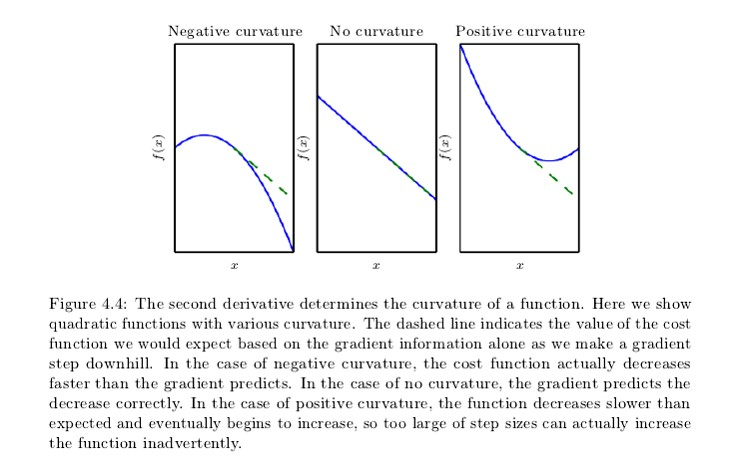
\includegraphics[width=6in]{fig/chap4/4_4.jpg} 
   \caption{图4.4
左:负曲率 中:零曲率 右:正曲率
图4.4:二次导数决定了函数的曲率。这里展示了二次函数的不同曲率。虚线表示了一个我们期望的只单一基于下降梯度变化的价值函数的值。在负曲率情况下,梯度下降的预测是正确的。在争取率的情况下,函数值降低要比期望更缓慢,甚至开始上升,多以过程的步长事实上会不慎使函数值上升。}
   \label{fig:4_4}
\end{figure}

\begin{equation}
\frac{\partial^2}{\partial x_j\partial x_i}f(x)=\frac{\partial^2}{\partial x_i\partial x_j}f(x)
\end{equation}

这就是说$H_{i,j}=H{j,i}$,所以海森矩阵在这样的点上是对称的。大多数我们在深度学习环境下遇到的函数全场都是对称海森矩阵。因为海森矩阵是真是的和对称的,我们可以分解为一组特征值和正交的基。在特定方向的二次导数由用$\vec{d}^T$Hd单位向量$\vec{d}$来表示.$\vec{d}$是H的特征向量,在这个方向的二阶导师由对应的特征向量给出。对于d的其他方向,方向性二阶微分是所有特征值的加权平均,系数从0到1,特征向量与d的方向夹角越小就有越高的系数。最大的特征值决定了最大的二阶导数,最小的特征值决定了最小的二阶导数。

二阶(方向)导数告诉了我们我们可以期望梯度下降执行的有多好(快慢)。我们可以对函数f(x)在瞬间点$x^{(0)}$做一个二阶泰勒级数近似:

\begin{equation}
f(x)\approx f(x^{(0)})+(x-x^{(0)})^Tg+\frac{1}{2}(x-x^{(0)})^TH(x-x^{(0)})
\end{equation}

在这里g是梯度,H是在$x^{(0)}$处的海森矩阵。如果我们使用学习速度$\epsilon$,新的点x就能够通过$x^{(0)}-\epsilon g$给出。将这个带入我们的近似,我们得到

\begin{equation}
f(x^{(0)}-\epsilon g)\approx f(x^{(0)})-\epsilon g^Tg+\frac{1}{2}\epsilon^2g^THg
\end{equation}

现在出现了三个术语:函数的原始值,由于斜率的函数预期值和由于曲率我们必须进一步修正的函数的值。当最后一项太过巨大时,梯度下降步骤可能上爬。当$g^THg$是零或者负值,泰勒展开近似预测$\epsilon$的永远增加会导致的永远减小。再练习中,泰勒级数在大$\epsilon$时不当像是能够保持精确,所以在这个问题中对$\epsilon$的取值我们要采取启发式的选择。当$g^THg$是正的,选择最优步长减少的泰勒级数近似最收益率的函数

\begin{equation}
\epsilon^*=\frac{g^Tg}{g^THg}
\end{equation}

在最糟糕的情况下,当g与对应H最大特征值$\lambda_{max}$的特征向量同向时,最优步长即为$\frac{1}{\lambda_{max}}$。直到我们去最小化的函数能够优秀地近似为二次函数,海森矩阵的特征值进而决定了学习速率。

二次导数可以用来确定临界点是局部最大,局部最小还是鞍点。记录在临界点上,
f'(x)=0.当f“(x)>0时表明在向左移动时f'(x)增加,同时当向右移动时f'(x)降低。这说明当$\epsilon$足够小的时候$f'(x-\epsilon)$<0并且$f'(x+\epsilon)$<0。换句话说,在我们向右移动时,斜率值向上坡,当我们向左移动时,斜率指向下坡。因此,当f'(x)=0当f“(x)>0我们能给出结论,x是局部最小值。相似的,当f'(x)=0.当f“(x)<0时,我们能得到x是局部最大值的结论。这被称作$\emph{二次导数检测}$。不幸的是,当f“(x)=0时,检测是无解的。在这个案例里的x可能是鞍点,或者是一个平台区域。

在多为中,我们需要检查函数的所有的二次导数。使用海森矩阵的特征分解,我们能多维空间的生成二次导数检测。在一个临界点,$\nabla_xf(x)=0$,我们能检测海森矩阵的特征值,来确定这个临界点是局部最大值,局部最小值还是鞍点。当海森矩阵一定是正的(所有的特征值均是正的),这个点就是局部最小值,这可以通过观察二阶方向导数在任何方向必须是正的,并且作为一元二次检测的参考。同样,当海森矩阵一定是为负(所有的特征值均为负)的时候,这个点就是最大点。在多维空间里,事实上在某些案例里可能能够找到鞍点为正的证据。当至少一个特征值是正的并且至少一个特征值是负的,我们知道在一个的样品里x是局部最大的,同时也是另一个样品里的局部最小值。见图4.5作为举例。最终,多维空间的二次导数测试是不确定的,就像一元样本。测试是不确定的,同时所有的非零特征值都有相同的迹象,但是至少一个特征值是零。这是因为单变量的二阶导数测试在样本特征值为零时是不确定的。

在多维空间里,在同一点可以有很多不同的二阶导数,因为在每个不同方向有不同的二阶导数。海森矩阵的条件数决定了二阶导数有多大的差异。当海森导数有很少的条件数时,梯度下降法执行很差。这是因为在一个方向上导数变化增加的迅速,同时在其他方向上,它增加的缓慢。梯度下降法不能够知道在导数上的这点变化,所以也不知道需要优先发现在一个倒数更长久的保持为负的方向上。这也是选择一个好的步长变得困难。步长大小必须足够小,来避免最小值过调或者由于强的正曲率导致在方向上爬升。这经常意味着步长大小要太小以至于不能在其他小曲率的方向上有显著的进展。见图4.6作为举例。

这个问题能够通过使用海森矩阵的信息来指导解决。这样做最简单的方法称作牛顿方法。牛顿方法是基于使用二阶泰勒级数展开来近似靠近点$x^{(0)}$:

\begin{equation}
f(x)\approx f(x^{(0)})+(x-x^{(0)})^T\nabla_xf(x^{(0)})+\frac{1}{2}(x-x^{(0)})^TH(f)(x^{(0)})(x-x^{(0)})
\end{equation}

当f是一个恒正的二次函数,牛顿方法包含方程4.12一次性直接将方程跳到最小值。当f不是二次函数的最小值但是可以局部近似成恒正二次函数,牛顿方法包括多次应用方程4.12.迭代更新近似值并且跳到近似的最小值这能够比梯度下降法更快地达到临界值。这在局部最小值是有意义的,但是在鞍点附近是有害的。在第8.2.3节中牛顿方法只有在靠近的临界点是最小值才近似(所有海森矩阵的特征值都是正的),然而梯度下降法则不会被鞍点吸引,除非梯度指向他们。

图\ref{fig:4_6}。
\begin{figure}[htbp] %  figure placement: here, top, bottom, or page
   \centering
   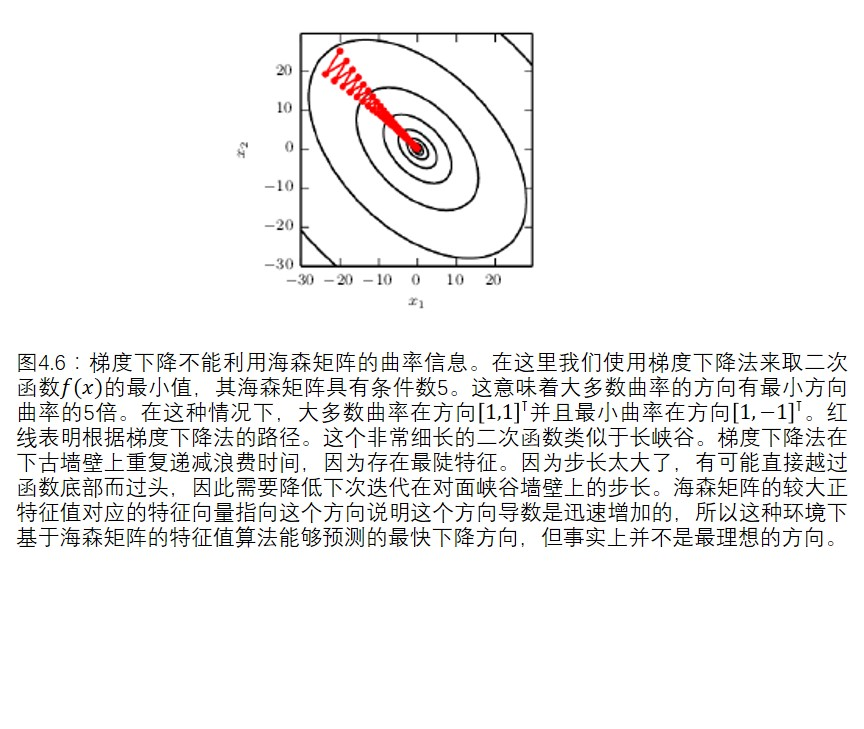
\includegraphics[width=6in]{fig/chap4/4_6.jpg} 
   \label{fig:4_6}
\end{figure}

优化算法,比如梯度下降法只是使用在称为一阶优化算法中。像诸如牛顿方法的算法也使用了海森矩阵,被称为$\emph{二阶优化算法}$.

优化算法使用在本书的大多数环境下适用于广泛种类的方程,甚至没有任何保证。这是因为应用在深度学习的方成家族是非常复杂的。在很多其他领域,接近最优化的域是为有限的方程去设计最优化算法。

在深度学习环境下,我们有时通过使用Lipschitz连续化或Lipschitz连续倒数限制我们自己构建方程并得到一些保证。Lipschitz连续函数就是变化率随着Lipschitz常数$\pounds$变化的函数:

\begin{equation}
\forall x,\forall y,\left | f(x)-f(y) \right |\leqslant\pounds\left \| x-y \right \|_2
\end{equation}

这个性质十分实用因为它允许我们去量化我们的假设,比如梯度下降法中,对于输入的微小改变会在输出也有一个小改变。Lipschitz连续是一个相当弱的约束,很多在深度学习中的优化问题可以与相当小的修改做Lipschitz连续。

也许专门的优化最好的使用领域是$\emph{凸优化}$。凸优化算法可以通过强约束避免许多保证。凸优化算法可以只能用于凸函数——海森矩阵各处都是半正定的。这样的函数行为良好,因为他们缺少鞍点并且他们所有的局部最小值必定是整体最小值。然而,大多数出现在深度学习中的问题都是很难用凸优化表示的。凸优化只用来作为一些深度学习算法的子程序。凸算法分析的想法能够对深度学习算法的收敛起有用的提升作用。然而,一般来说,凸算法的重要性在深度学习环境下是大幅衰减的。对于更多凸优化的信息,见Boyd and Vandenberghe(2004) or Rockafellar(1997).

图\ref{fig:4_5}。
\begin{figure}[htbp] %  figure placement: here, top, bottom, or page
   \centering
   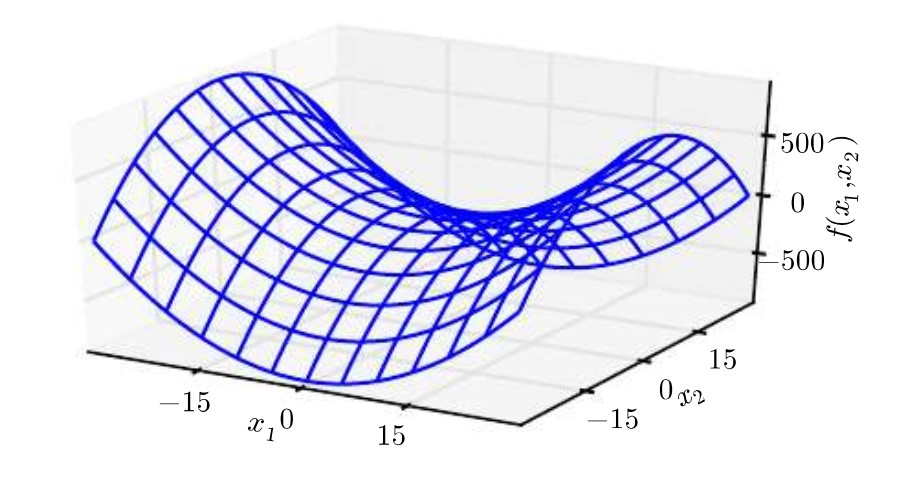
\includegraphics[width=6in]{fig/chap4/4_5.jpg} 
   \caption{图4.5:一个鞍点位置同时包含正曲率和负曲率。该例子所用的函数为f(x)=$x_1^2-x_2^2$。沿着$x_1$坐标轴方向,函数是向上弯曲(开口向上),该轴是H的一个特征向量,对应了一个正特征值。同理,沿着$x_2$坐标轴方向,函数是向下弯曲(开口向下),该轴是H的一个特征向量,对应了一个负特征值。鞍点因该点形状类似马鞍而得名。该函数是鞍点一个非常妙的例子。在更高的维度中,不必再通过拥有0特征值来找到鞍点:只需要同时拥有正特征值和负特征值即可。我们可以认为鞍点在对应两个特征值的两个特征向量的方向上,一个截面内是极小值,另一个截面内是极大值。}
   \label{fig:4_5}
\end{figure}



\section{4.0}